\chapter{Buffers en predominantiediagrammen}\label{ch:g12:buffers-predominance}

Een bloedonderzoek geeft de \omterm{def:g9:acids-bases-ph:ph}{pH} van arterieel bloed: normaal tussen 7.38 en
7.42. Werkende spieren storten zuren in het bloed, de longen blazen er
koolstofdioxide uit, voedsel brengt zuren en basen binnen; toch beweegt
de \omterm{def:g9:acids-bases-ph:ph}{pH} nauwelijks. Een paar deeltjes, een zuur en zijn eigen base, vangt
die schokken op. Dit hoofdstuk laat zien welke vorm van een koppel bij een
gegeven \omterm{def:g9:acids-bases-ph:ph}{pH} overheerst, hoe een paar druppels van een gekleurd koppel de
\omterm{def:g9:acids-bases-ph:ph}{pH} verraden, en hoe een \omterm{def:g6:pure-substances-and-mixtures:mixture}{mengsel} van een zuur en zijn base de \omterm{def:g9:acids-bases-ph:ph}{pH} stabiel
houdt.

\begin{recall}
\omterm{def:g12:ka-and-pka:bronsted}{Zuur-basekoppels}, $K_a$ en $pK_a$; de \omterm{def:g9:acids-bases-ph:ph}{pH} van een oplossing
(\cref{ch:g12:ka-and-pka}, \cref{ch:g9:acids-bases-ph}).
\end{recall}

\begin{omfigure}
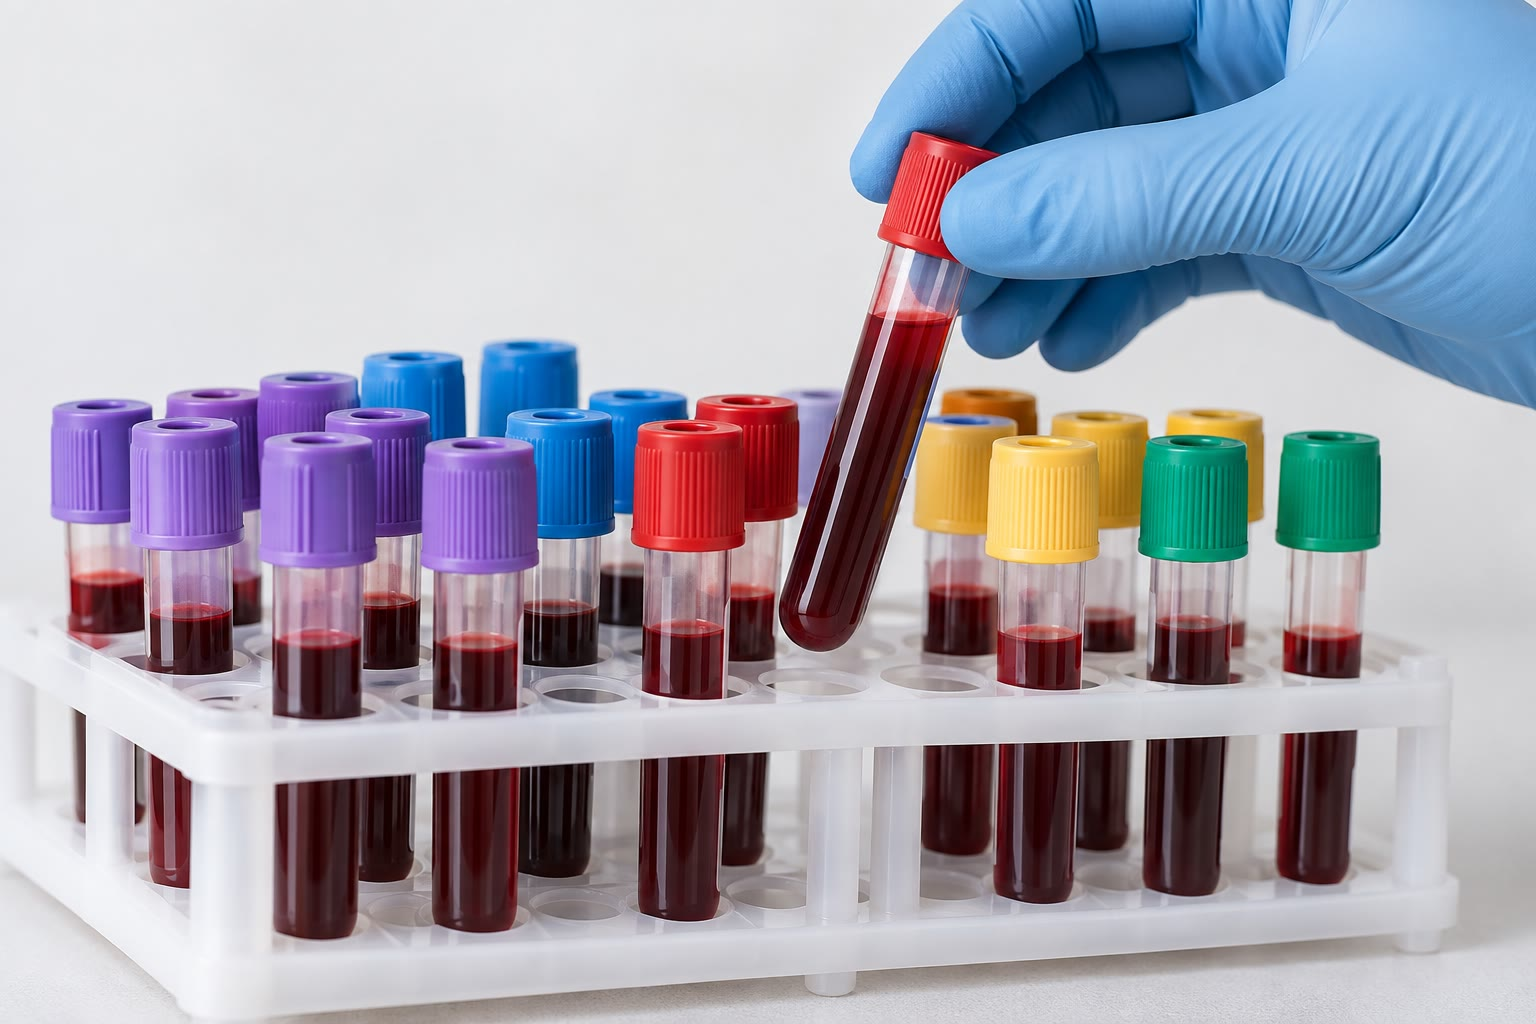
\includegraphics[width=0.45\linewidth]{images/book1/ai/g12-blood-tubes.jpg}

{\small Bloedmonsters: hun \omterm{def:g9:acids-bases-ph:ph}{pH} wordt binnen een smal gebied gehouden.}
\end{omfigure}

\section{Predominantiediagrammen}

\begin{proposition}[De betrekking van Henderson]\label{prop:g12:buffers-predominance:henderson}
In elke \omterm{def:g6:solutions-and-solubility:solute}{waterige oplossing} die het koppel \ce{HA}/\ce{A-} bevat, geldt
\[
  \mathrm{pH} = pK_a + \log\frac{[\ce{A-}]}{[\ce{HA}]} .
\]
\end{proposition}

\begin{proof}
Neem van beide kanten van $K_a = \dfrac{[\ce{A-}][\ce{H3O+}]}{[\ce{HA}]c^\circ}$
de $-\log$:
$pK_a = \mathrm{pH} - \log\dfrac{[\ce{A-}]}{[\ce{HA}]}$.
\end{proof}

\begin{definition}[Predominantie- en verdelingsdiagrammen]\label{def:g12:buffers-predominance:predominance}
Het \emph{predominantiediagram}\index{predominantiediagram} van een koppel
is een pH-as die bij $pK_a$ in tweeën is gedeeld: daaronder overheerst het
zuur HA ($[\ce{HA}] > [\ce{A-}]$), daarboven de base \ce{A-}. Het
\emph{verdelingsdiagram}\index{verdelingsdiagram} laat het aandeel van
elke vorm zien,
$[\ce{HA}]/c$ en $[\ce{A-}]/c$, tegen de \omterm{def:g9:acids-bases-ph:ph}{pH}; de twee krommen snijden
elkaar bij
$\mathrm{pH} = pK_a$.
\end{definition}

\begin{method}[Een predominantiediagram tekenen]\label{met:g12:buffers-predominance:diagram}
\begin{enumerate}
  \item Teken een pH-as van 0 tot 14 en geef de $pK_a$ van het koppel
        aan.
  \item Schrijf het zuur links van $pK_a$ en de base rechts.
  \item Geef voor een deeltje met meerdere koppels (een zuur dat twee
        waterstofionen kan afstaan, een aminozuur) elke $pK_a$ aan: elk
        interval hoort bij één vorm.
  \item Eén eenheid van $pK_a$ af is de verhouding al 10 op 1: de kleinste
        vorm zit onder \qty{10}{\percent}.
\end{enumerate}
\end{method}

\begin{omfigure}
\begin{tikzpicture}[font=\small, x=0.62cm]
  % ledger: pka:ethanoic, pka:methanoic, kb:NH3, ka:H2CO3
  \foreach \y/\pk/\acid/\base in {0/3.74/{\ce{HCOOH}}/{\ce{HCOO-}},
      -1.0/4.76/{\ce{CH3COOH}}/{\ce{CH3COO-}}, -2.0/6.37/{\ce{CO2,H2O}}/{\ce{HCO3-}},
      -3.0/9.26/{\ce{NH4+}}/{\ce{NH3}}} {
    \fill[omThm!20] (0,\y) rectangle (\pk,\y+0.5);
    \fill[omDef!20] (\pk,\y) rectangle (14,\y+0.5);
    \draw[black!50] (0,\y) rectangle (14,\y+0.5);
    \node at (\pk/2,\y+0.25) {\acid};
    \node at ({(\pk+14)/2},\y+0.25) {\base};
    \draw[thick] (\pk,\y-0.08) -- (\pk,\y+0.58);
    \node[font=\scriptsize, anchor=south] at (\pk,\y+0.55) {\pk};
  }
  \draw[->] (0,-3.4) -- (14.5,-3.4) node[right] {pH};
  \foreach \k in {0,2,4,6,8,10,12,14} \draw (\k,-3.35) -- (\k,-3.45) node[below, font=\scriptsize] {\k};
\end{tikzpicture}

{\small \omterm{def:g12:buffers-predominance:predominance}{Predominantiediagrammen} van vier koppels: het zuur (links, rood)
overheerst onder zijn $pK_a$, de base (rechts, blauw) erboven.}
\end{omfigure}

\begin{omfigure}
\begin{minipage}{0.49\linewidth}
\begin{tikzpicture}
\begin{axis}[width=\linewidth, height=5cm, xmin=0, xmax=14, ymin=0, ymax=1.05,
    xlabel={pH}, ylabel={aandeel}, axis lines*=left, ymajorgrids,
    grid style={gray!20}, tick label style={font=\scriptsize},
    label style={font=\small}, title={\small ethaanzuur},
    title style={yshift=-4pt}]
  \addplot[very thick, omThm] table[x=pH, y=HA] {figdata/out/grade-12-buffers-predominance-a.dat};
  \addplot[very thick, omDef] table[x=pH, y=A] {figdata/out/grade-12-buffers-predominance-a.dat};
  \addplot[dashed, black!50] coordinates {(4.76,0) (4.76,1)};
  \node[font=\scriptsize, omThm] at (axis cs:2.2,0.85) {\ce{CH3COOH}};
  \node[font=\scriptsize, omDef] at (axis cs:7.6,0.85) {\ce{CH3COO-}};
\end{axis}
\end{tikzpicture}
\end{minipage}\hfill
\begin{minipage}{0.49\linewidth}
\begin{tikzpicture}
\begin{axis}[width=\linewidth, height=5cm, xmin=0, xmax=14, ymin=0, ymax=1.05,
    xlabel={pH}, ylabel={aandeel}, axis lines*=left, ymajorgrids,
    grid style={gray!20}, tick label style={font=\scriptsize},
    label style={font=\small}, title={\small glycine},
    title style={yshift=-4pt}]
  \addplot[very thick, omThm] table[x=pH, y=cation] {figdata/out/grade-12-buffers-predominance-b.dat};
  \addplot[very thick, omMeth] table[x=pH, y=zwitterion] {figdata/out/grade-12-buffers-predominance-b.dat};
  \addplot[very thick, omDef] table[x=pH, y=anion] {figdata/out/grade-12-buffers-predominance-b.dat};
  \node[font=\scriptsize, omThm] at (axis cs:1.0,0.55) {kation};
  \node[font=\scriptsize, omMeth] at (axis cs:6.1,0.88) {zwitterion};
  \node[font=\scriptsize, omDef] at (axis cs:12.6,0.55) {anion};
\end{axis}
\end{tikzpicture}
\end{minipage}

{\small \omterm{def:g12:buffers-predominance:predominance}{Verdelingsdiagrammen}, berekend uit de $pK_a$-waarden. Links:
ethaanzuur, de krommen snijden elkaar bij 4.76. Rechts: glycine,
\ce{H2N-CH2-COOH}, met twee koppels ($pK_a$ 2.35 en 9.78): het \omterm{def:g9:ions:ion}{kation}
\ce{H3N+-CH2-COOH}, het zwitterion \ce{H3N+-CH2-COO-} en het \omterm{def:g9:ions:ion}{anion}
\ce{H2N-CH2-COO-}.}
\end{omfigure}

\begin{example}[Glycine in het lichaam]\label{ex:g12:buffers-predominance:glycine}
% ledger: pka:glycine1, pka:glycine2, ph:blood
Bij de \omterm{def:g9:acids-bases-ph:ph}{pH} van bloed, ongeveer 7.4, ligt glycine tussen zijn twee
$pK_a$-waarden: het is bijna helemaal in de vorm van het zwitterion, met
een positieve lading op zijn stikstofatoom en een negatieve lading op zijn
carboxylaatgroep, en als geheel neutraal. Elk aminozuur gedraagt zich zo.
\end{example}

\section{Zuur-base-indicatoren}


\begin{definition}[Zuur-base-indicator, omslagtraject]\label{def:g12:buffers-predominance:indicator}
Een \emph{zuur-base-indicator}\index{zuur-base-indicator} is een koppel
\ce{HInd}/\ce{Ind-} waarvan de twee vormen verschillende kleuren hebben,
en dat in heel kleine hoeveelheden gebruikt wordt. Het
\emph{omslagtraject}\index{omslagtraject} is het pH-interval waarin je de
kleur ziet omslaan, ruwweg van
$pK_a - 1$ tot $pK_a + 1$: daaronder zie je de kleur van \ce{HInd},
daarboven die van \ce{Ind-}, en daartussen een \omterm{def:g6:pure-substances-and-mixtures:mixture}{mengsel} van beide.
\end{definition}

\begin{omfigure}
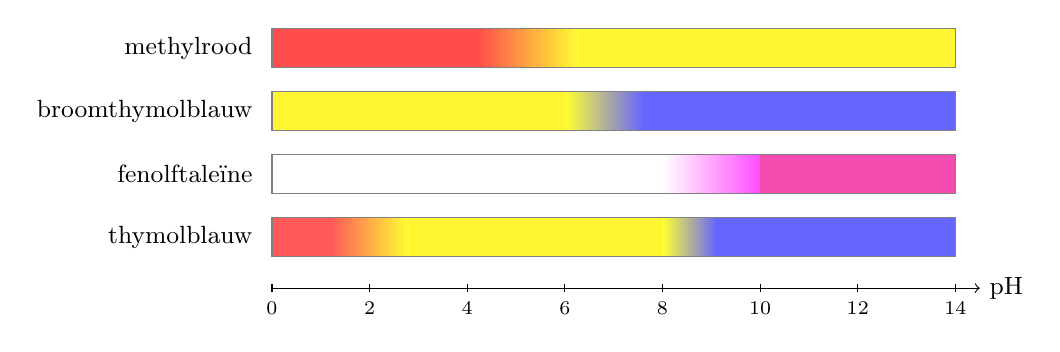
\begin{tikzpicture}[font=\small, x=0.62cm]
  % ledger: ind:methyl-red, ind:BBT, ind:phenolphthalein, ind:thymol-blue, ind:range-rule
  \foreach \y/\name/\a/\b/\ca/\cm/\cb in {
      0/{methylrood}/4.2/6.3/red!70/orange/yellow!80,
      -0.8/{broomthymolblauw}/6.0/7.6/yellow!80/green!60/blue!60,
      -1.6/{fenolftaleïne}/8.0/10.0/white/magenta!25/magenta!70} {
    \fill[\ca] (0,\y) rectangle (\a,\y+0.5);
    \shade[left color=\ca, right color=\cb] (\a,\y) rectangle (\b,\y+0.5);
    \fill[\cb] (\b,\y) rectangle (14,\y+0.5);
    \draw[black!50] (0,\y) rectangle (14,\y+0.5);
    \node[anchor=east] at (-0.2,\y+0.25) {\name};
  }
  \fill[red!65] (0,-2.4) rectangle (1.2,-1.9);
  \shade[left color=red!65, right color=yellow!80] (1.2,-2.4) rectangle (2.8,-1.9);
  \fill[yellow!80] (2.8,-2.4) rectangle (8.0,-1.9);
  \shade[left color=yellow!80, right color=blue!60] (8.0,-2.4) rectangle (9.1,-1.9);
  \fill[blue!60] (9.1,-2.4) rectangle (14,-1.9);
  \draw[black!50] (0,-2.4) rectangle (14,-1.9);
  \node[anchor=east] at (-0.2,-2.15) {thymolblauw};
  \draw[->] (0,-2.8) -- (14.5,-2.8) node[right] {pH};
  \foreach \k in {0,2,4,6,8,10,12,14} \draw (\k,-2.75) -- (\k,-2.85) node[below, font=\scriptsize] {\k};
\end{tikzpicture}

{\small Kleuren van vier indicatoren tegen de \omterm{def:g9:acids-bases-ph:ph}{pH}; de gearceerde stukken
zijn de \omterm{def:g12:buffers-predominance:indicator}{omslagtrajecten}. Thymolblauw, met twee koppels, heeft twee
\omterm{def:g12:buffers-predominance:indicator}{omslagtrajecten}.}
\end{omfigure}

\begin{method}[Een indicator kiezen]\label{met:g12:buffers-predominance:indicator}
Om te zien wanneer een oplossing een bepaalde \omterm{def:g9:acids-bases-ph:ph}{pH} passeert (bijvoorbeeld
de \omterm{def:g9:acids-bases-ph:ph}{pH} aan het eind van een \omterm{def:g11:titration:titration}{titratie}), kies je een indicator waarvan het
\omterm{def:g12:buffers-predominance:indicator}{omslagtraject} die \omterm{def:g9:acids-bases-ph:ph}{pH} bevat: de kleur slaat dan precies daar om.
\end{method}

\section{Bufferoplossingen}

\begin{definition}[Bufferoplossing]\label{def:g12:buffers-predominance:buffer}
Een \emph{bufferoplossing}\index{bufferoplossing} is een oplossing
waarvan de \omterm{def:g9:acids-bases-ph:ph}{pH} heel weinig verandert als er een beetje zuur of base wordt
toegevoegd, of als ze verdund wordt. Ze bestaat meestal uit een \omterm{def:g12:ka-and-pka:strong-acid}{zwak zuur}
en zijn geconjugeerde base in vergelijkbare hoeveelheden; haar \omterm{def:g9:acids-bases-ph:ph}{pH} ligt
dan dicht bij de $pK_a$ van het koppel.
\end{definition}

\begin{proposition}[Waarom een buffer weerstand biedt]\label{prop:g12:buffers-predominance:buffer}
In een buffer van \ce{HA} en \ce{A-} wordt een toegevoegd \omterm{def:g12:ka-and-pka:strong-acid}{sterk zuur}
verbruikt door
\ce{A-} (\ce{A- + H3O+ -> HA + H2O}) en een toegevoegde \omterm{def:g12:ka-and-pka:strong-acid}{sterke base} door
\ce{HA} (\ce{HA + OH- -> A- + H2O}); de verhouding $[\ce{A-}]/[\ce{HA}]$,
en dus de \omterm{def:g9:acids-bases-ph:ph}{pH}, verandert maar weinig. Verdunnen verandert de verhouding
helemaal niet.
\end{proposition}

\begin{proof}
Volgens de betrekking van Henderson hangt de \omterm{def:g9:acids-bases-ph:ph}{pH} alleen af van de
verhouding. Als je \qty{1}{mmol} zuur toevoegt aan een buffer met
\qty{10}{mmol} van elke vorm, verandert de verhouding van $10/10$ in
$9/11$, en de \omterm{def:g9:acids-bases-ph:ph}{pH} met maar
$\log(9/11) = -0.09$.
\end{proof}

\begin{omfigure}
\begin{tikzpicture}
\begin{axis}[width=0.75\linewidth, height=5.6cm, xmin=0, xmax=10, ymin=0,
    ymax=8, xlabel={toegevoegd \ce{HCl} van \qty{0.10}{mol/L} (\si{mL})},
    ylabel={pH}, axis lines*=left, ymajorgrids, grid style={gray!20},
    tick label style={font=\small}, label style={font=\small},
    legend style={font=\small, at={(0.98,0.97)}, anchor=north east,
    draw=none, fill=white}, legend cell align=left]
  % ledger: pka:ethanoic (buffer recipe: exercise data)
  \addplot[very thick, omThm, mark=*, mark size=1.3pt] table[x=V, y=water]
    {figdata/out/grade-12-buffers-predominance-c.dat};
  \addplot[very thick, omDef, mark=*, mark size=1.3pt] table[x=V, y=buffer]
    {figdata/out/grade-12-buffers-predominance-c.dat};
  \legend{\qty{100}{mL} zuiver water, \qty{100}{mL} ethanoaatbuffer}
\end{axis}
\end{tikzpicture}

{\small Zoutzuur toevoegen aan zuiver water en aan een buffer van
ethaanzuur en natriumethanoaat (elk \qty{0.10}{mol/L}). De \omterm{def:g9:acids-bases-ph:ph}{pH} van water
daalt van 7 tot ongeveer 2; die van de buffer van 4.76 tot 4.67.}
\end{omfigure}

\begin{method}[Een buffer maken]\label{met:g12:buffers-predominance:prepare}
\begin{enumerate}
  \item Kies een koppel waarvan de $pK_a$ minder dan één eenheid van de
        gewenste \omterm{def:g9:acids-bases-ph:ph}{pH} af ligt (het liefst er vlak bij).
  \item Bereken de verhouding $[\ce{A-}]/[\ce{HA}] = 10^{\mathrm{pH} - pK_a}$.
  \item Meng het \omterm{def:g12:ka-and-pka:strong-acid}{zwakke zuur} en een zout van zijn base in die verhouding,
        in concentraties die hoog genoeg zijn om de hoeveelheden zuur of
        base op te vangen.
\end{enumerate}
\end{method}

\begin{inthelab}[Een buffer van pH 4.8 maken]
\qty{50.0}{mL} ethaanzuur van \qty{0.10}{mol/L} wordt gemengd met
\qty{50.0}{mL} natriumethanoaat van \qty{0.10}{mol/L}; een \omterm{def:g9:acids-bases-ph:ph-paper}{pH-meter} geeft
ongeveer 4.8 aan. Een paar druppels zoutzuur van \qty{1}{mol/L} laten de
aflezing nauwelijks bewegen, terwijl dezelfde druppels in \qty{100}{mL}
gedestilleerd water haar tot ongeveer 3 laten dalen.
\end{inthelab}

\section{Buffers in levende wezens}

\begin{example}[De buffer van het bloed]\label{ex:g12:buffers-predominance:blood}
% ledger: pk:blood-bicarb, ph:blood, hco3:blood
De belangrijkste buffer van bloed is het koppel van opgelost
koolstofdioxide en het waterstofcarbonaation, \ce{CO2,H2O}/\ce{HCO3-}.
Voor bloed gebruiken fysiologen daarvoor de betrekking $\mathrm{pH} = 6.1 +
\log\big([\ce{HCO3-}]/[\ce{CO2}]\big)$. De longen verwijderen
koolstofdioxide, de nieren regelen het waterstofcarbonaat bij: samen
houden ze de verhouding, en dus de \omterm{def:g9:acids-bases-ph:ph}{pH}, vast.
\end{example}

\begin{omfigure}
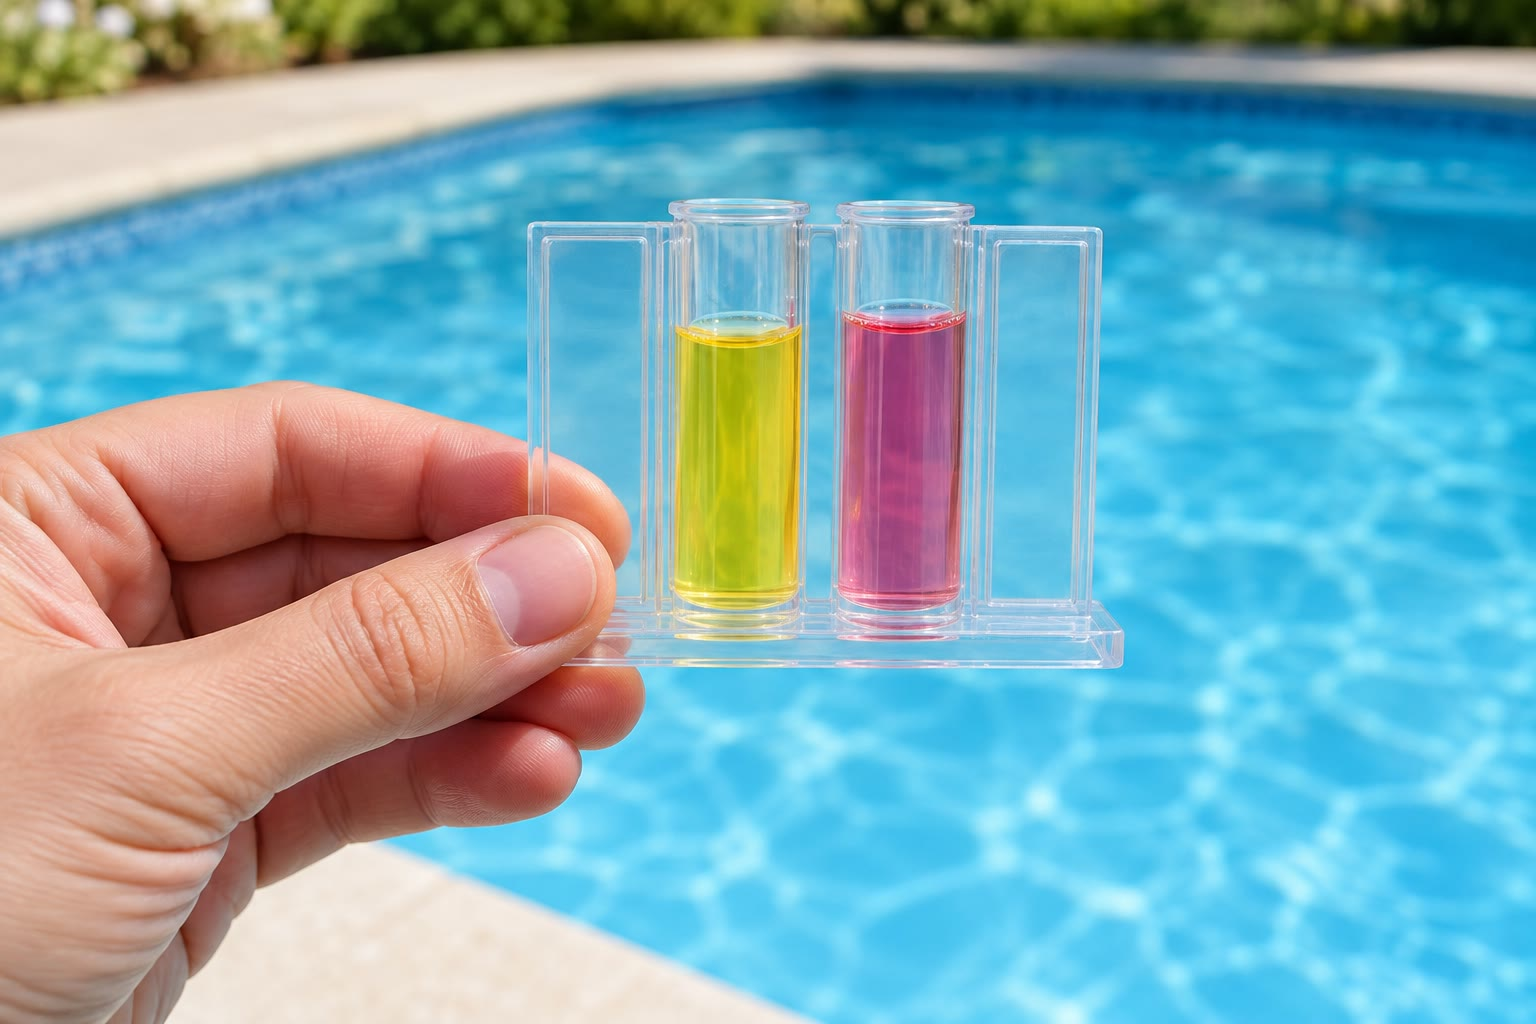
\includegraphics[width=0.45\linewidth]{images/book1/ai/g12-pool-test.jpg}

{\small Zwembadwater testen: de kleuren van indicatoren geven de \omterm{def:g9:acids-bases-ph:ph}{pH}.}
\end{omfigure}

\section{Oefeningen}


\begin{exercise}[$\star$]\label{exo:g12:buffers-predominance:1}
Welke vorm van het koppel \ce{CH3COOH}/\ce{CH3COO-} ($pK_a = 4.76$)
overheerst bij \omterm{def:g9:acids-bases-ph:ph}{pH} 2, bij \omterm{def:g9:acids-bases-ph:ph}{pH} 4.76 en bij \omterm{def:g9:acids-bases-ph:ph}{pH} 7?
\end{exercise}

\begin{exercise}[$\star$]\label{exo:g12:buffers-predominance:2}
Lees in het \omterm{def:g12:buffers-predominance:predominance}{verdelingsdiagram} van ethaanzuur het aandeel \ce{CH3COO-} af
bij \omterm{def:g9:acids-bases-ph:ph}{pH} 4 en bij \omterm{def:g9:acids-bases-ph:ph}{pH} 6.
\end{exercise}

\begin{exercise}[$\star$]\label{exo:g12:buffers-predominance:3}
Welke kleur heeft broomthymolblauw bij \omterm{def:g9:acids-bases-ph:ph}{pH} 5? Bij \omterm{def:g9:acids-bases-ph:ph}{pH} 7? Bij \omterm{def:g9:acids-bases-ph:ph}{pH} 9?
\end{exercise}

\begin{exercise}[$\star$]\label{exo:g12:buffers-predominance:4}
Welke vorm van het koppel \ce{NH4+}/\ce{NH3} overheerst in een oplossing
met \omterm{def:g9:acids-bases-ph:ph}{pH} 7.4? Met \omterm{def:g9:acids-bases-ph:ph}{pH} 11?
\end{exercise}

\begin{exercise}[$\star$]\label{exo:g12:buffers-predominance:5}
Waarom gebruikt men indicatoren in heel kleine hoeveelheden?
\end{exercise}

\begin{exercise}[$\star\star$]\label{exo:g12:buffers-predominance:6}
Bereken de verhouding $[\ce{CH3COO-}]/[\ce{CH3COOH}]$ bij \omterm{def:g9:acids-bases-ph:ph}{pH} 3.76, 4.76 en
5.76.
\end{exercise}

\begin{exercise}[$\star\star$]\label{exo:g12:buffers-predominance:7}
Een \omterm{def:g11:titration:titration}{titratie} eindigt bij \omterm{def:g9:acids-bases-ph:ph}{pH} 8.7. Welke van de vier indicatoren uit de
figuur zou je kiezen? Waarom niet methylrood?
\end{exercise}

\begin{exercise}[$\star\star$]\label{exo:g12:buffers-predominance:8}
Een buffer bevat \qty{0.20}{mol/L} ethaanzuur en \qty{0.10}{mol/L}
natriumethanoaat. Bereken de \omterm{def:g9:acids-bases-ph:ph}{pH} ervan.
\end{exercise}

\begin{exercise}[$\star\star$]\label{exo:g12:buffers-predominance:9}
Geef met het diagram van glycine de overheersende vorm bij \omterm{def:g9:acids-bases-ph:ph}{pH} 1, 6 en 12,
met de lading ervan.
\end{exercise}

\begin{exercise}[$\star\star$]\label{exo:g12:buffers-predominance:10}
Lees de responskrommen af: hoeveel daalt de \omterm{def:g9:acids-bases-ph:ph}{pH} van water na
\qty{1.0}{mL} zuur? En die van de buffer?
\end{exercise}

\begin{exercise}[$\star\star$]\label{exo:g12:buffers-predominance:11}
Welk koppel uit de figuur met \omterm{def:g12:buffers-predominance:predominance}{predominantiediagrammen} zou je kiezen om een
buffer van \omterm{def:g9:acids-bases-ph:ph}{pH} 9.5 te maken? In welke verhouding zou je de twee vormen
\omterm{def:g2:mixing-and-dissolving:mix}{mengen}?
\end{exercise}

\begin{exercise}[$\star\star\star$]\label{exo:g12:buffers-predominance:12}
De ethanoaatbuffer uit de figuur (\qty{10}{mmol} van elke vorm) krijgt
zoutzuur toegevoegd. Hoeveel zuur kan hij opnemen voordat zijn \omterm{def:g9:acids-bases-ph:ph}{pH} met één
eenheid gedaald is? Waarom zegt men dat een geconcentreerdere buffer een
grotere capaciteit heeft?
\end{exercise}

\begin{exercise}[$\star\star\star$]\label{exo:g12:buffers-predominance:13}
Welk volume oplossing van natriumethanoaat van \qty{0.10}{mol/L} moet je
toevoegen aan \qty{100}{mL} ethaanzuur van \qty{0.10}{mol/L} om een buffer
van \omterm{def:g9:acids-bases-ph:ph}{pH} 5.0 te krijgen?
\end{exercise}

\begin{exercise}[$\star\star\star$]\label{exo:g12:buffers-predominance:14}
Thymolblauw heeft twee \omterm{def:g12:buffers-predominance:indicator}{omslagtrajecten}. Leg uit waarom, en geef de kleur
ervan bij \omterm{def:g9:acids-bases-ph:ph}{pH} 1, 5 en 10.
\end{exercise}

\begin{exercise}[$\star\star\star$]\label{exo:g12:buffers-predominance:15}
Een buffer van \omterm{def:g9:acids-bases-ph:ph}{pH} 4.76 wordt tien keer verdund met gedestilleerd water.
Wat is volgens de betrekking van Henderson zijn nieuwe \omterm{def:g9:acids-bases-ph:ph}{pH}? Wat gebeurt er
als een \omterm{def:g12:ka-and-pka:strong-acid}{sterk zuur} met dezelfde \omterm{def:g9:acids-bases-ph:ph}{pH} tien keer verdund wordt?
\end{exercise}

\section{Probleem: De buffer van het bloed}

\begin{problem}[{Weekendprobleem --- welke verhouding tussen
waterstofcarbonaat en koolstofdioxide houdt bloed op pH 7.4?}]
\label{pb:g12:buffers-predominance:1}
% ledger: pk:blood-bicarb, ph:blood, hco3:blood
De \omterm{def:g9:acids-bases-ph:ph}{pH} van arterieel bloed ligt normaal tussen 7.38 en 7.42. De
belangrijkste buffer is het koppel \ce{CO2,H2O}/\ce{HCO3-}, waarvoor
fysiologen
$\mathrm{pH} = 6.1 + \log\big([\ce{HCO3-}]/[\ce{CO2}]\big)$ gebruiken. De
normale concentratie waterstofcarbonaat in bloed is 22 tot
\qty{28}{mmol/L}.

\medskip
\noindent\textbf{Deel I --- Het koppel.}
\begin{enumerate}
  \item Schrijf de reactie op van opgelost koolstofdioxide met water,
        waarbij waterstofcarbonaationen ontstaan.
  \item Welk deeltje is het zuur, welk de base?
  \item De waarde 6.1 verschilt van de 6.37 uit de tabel van
        $pK_a$-waarden. Geef een reden (denk aan de temperatuur van het
        lichaam en aan de andere \omterm{def:g9:ions:ion}{ionen} die aanwezig zijn).
  \item Welke hoeveelheid waterstofcarbonaat bevat \qty{5.0}{L} bloed
        bij \qty{24}{mmol/L}?
\end{enumerate}

\medskip
\noindent\textbf{Deel II --- Predominantie.}
\begin{enumerate}[resume]
  \item Teken het \omterm{def:g12:buffers-predominance:predominance}{predominantiediagram} van het koppel met $pK = 6.1$.
  \item Welke vorm overheerst in bloed?
  \item Is bloed licht zuur of licht basisch?
\end{enumerate}

\medskip
\noindent\textbf{Deel III --- De verhouding.}
\begin{enumerate}[resume]
  \item Bereken met de betrekking de verhouding $[\ce{HCO3-}]/[\ce{CO2}]$
        bij \omterm{def:g9:acids-bases-ph:ph}{pH} 7.4.
  \item Neem $[\ce{HCO3-}] = \qty{24}{mmol/L}$ en bereken $[\ce{CO2}]$.
  \item Bereken de verhouding aan de twee uiteinden van het normale
        gebied, 7.38 en 7.42.
  \item Welk deel van het koppel is bij \omterm{def:g9:acids-bases-ph:ph}{pH} 7.4 in de vorm van
        waterstofcarbonaat?
  \item Bloed dat te basisch is, kan \omterm{def:g9:acids-bases-ph:ph}{pH} 7.6 bereiken. Wat is de
        verhouding dan?
\end{enumerate}

\medskip
\noindent\textbf{Deel IV --- Als het evenwicht verloren gaat.}
\begin{enumerate}[resume]
  \item Bij een zware inspanning komen er zuren in het bloed. Welke vorm
        van het koppel verbruikt ze? Schrijf de reactie op.
  \item Wat zou de verhouding worden als de \omterm{def:g9:acids-bases-ph:ph}{pH} tot 7.1 daalde?
  \item Hoeveel zou het koolstofdioxide moeten toenemen bij een
        ongewijzigde hoeveelheid waterstofcarbonaat? Wat doen de longen om
        terug te vechten?
  \item Waarom is een \omterm{def:g12:ka-and-pka:strong-acid}{zwak zuur} met zijn base, en niet een \omterm{def:g12:ka-and-pka:strong-acid}{sterk zuur}, het
        juiste middel om een \omterm{def:g9:acids-bases-ph:ph}{pH} vast te houden?
  \item Hoeveel verandert de \omterm{def:g9:acids-bases-ph:ph}{pH} als beide concentraties door twee worden
        gedeeld? Waarom?
  \item Geef het eindantwoord: wat is de verhouding tussen
        waterstofcarbonaat en koolstofdioxide in bloed bij \omterm{def:g9:acids-bases-ph:ph}{pH} 7.4?
\end{enumerate}
\end{problem}
